\documentclass[a4paper,14pt]{extarticle} 
\usepackage[a4paper,top=1.5cm, bottom=1.5cm, left=2cm, right=1cm]{geometry}
%\usepackage[T2A]{fontenc}
%\usepackage[english, russian]{babel}
\usepackage{graphicx}
\DeclareGraphicsExtensions{.pdf,.png,.jpg}

\usepackage{fontspec}
\setmainfont{Times New Roman}
\setsansfont{FreeSans}
\setmonofont{FreeMono}
\renewcommand{\baselinestretch}{1.5}
\usepackage{polyglossia}
\setdefaultlanguage{russian}
\setotherlanguages{english,russian}
\usepackage{setspace}
\usepackage[many]{tcolorbox}
\usepackage{listings}
\usepackage{xcolor}

\definecolor{codegreen}{rgb}{0,0.6,0}
\definecolor{codegray}{rgb}{0.5,0.5,0.5}
\definecolor{codepurple}{rgb}{0.58,0,0.82}
\definecolor{backcolour}{rgb}{0.95,0.95,0.92}

\lstdefinestyle{mystyle}{
    backgroundcolor=\color{backcolour},   
    keywordstyle=\color{magenta},
    numberstyle=\tiny\color{codegray},
    stringstyle=\color{codepurple},
    basicstyle=\ttfamily\footnotesize,
    breakatwhitespace=false,         
    breaklines=true,                 
    captionpos=b,                    
    keepspaces=true,                 
    numbers=left,                    
    numbersep=5pt,                  
    showspaces=false,                
    showstringspaces=false,
    showtabs=false,                  
    tabsize=2
}

\lstset{style=mystyle}
\setlength{\parindent}{5ex}


\begin{document}
    \begin{center}
        \thispagestyle{empty}
        \begin{singlespace}
        ФЕДЕРАЛЬНОЕ АГЕНТСТВО СВЯЗИ

        ФЕДЕРАЛЬНОЕ ГОСУДАРСТВЕННОЕ БЮДЖЕТНОЕ ОБРАЗОВАТЕЛЬНОЕ

        УЧРЕЖДЕНИЕ ВЫСШЕГО ОБРАЗОВАНИЯ

        «САНКТ-ПЕТЕРБУРГСКИЙ ГОСУДАРСТВЕННЫЙ УНИВЕРСИТЕТ ТЕЛЕКОММУНИКАЦИЙ ИМ. ПРОФ. М.А. БОНЧ-БРУЕВИЧА»

        (СПбГУТ)
        \end{singlespace}
        \vspace{-1ex}
        \rule{\textwidth}{0.4pt}
        \vspace{-5ex}

        Факультет \underline{Инфокоммуникационных сетей и систем}

        Кафедра \underline{Защищенных систем связи}
        \vspace{10ex}

        \textbf{Лаборатоoрная работа №2}\\
        МОНИТОРИНГ СЕТЕВОЙ И КОМПЬЮТЕРНОЙ АКТИВНОСТИ ПОЛЬЗОВАТЕЛЕЙ. Ч.2
        


    \end{center}
    \vspace{4ex}
    \begin{flushright}
    \parbox{10 cm}{
    \begin{flushleft}
        Выполнили студенты группы ИКТЗ-83:

        \underline{Громов А.А., Миколаени М.С., Мазеин Д.С.} \hfill \rule[-0.85ex]{0.1\textwidth}{0.6pt}

        \footnotesize \textit{ (Ф.И.О., № группы) \hfill (подпись)} \normalsize

        Проверил:

        \underline{Казанцев А.А.} \hfill \rule[-0.85ex]{0.1\textwidth}{0.6pt}

        (\footnotesize \textit{уч. степень, уч. звание, Ф.И.О.) \hfill (подпись)} \normalsize

    \end{flushleft}
    }
    \end{flushright}
    \begin{center}
        \vfill
        Санкт-Петербург

        2021

    \end{center}
    \newpage

    \textbf{Цель лабораторной работы:}

    Научиться работе с Клиентской консолью Falcongaze SecureTower для проведения расследований и предупреждения инцидентов
    информационной безопасности организации, освоить инструмент создания статистических отчетов о компьютерной и сетевой активности 
    пользователей. Научиться использовать инструменты системы для наблюдения за активностью пользователей в режиме реального времени 
    и для мониторинга файловых систем.

    \textbf{Пункт 2.4 - Дублирование отчета.} 
    \begin{center}
        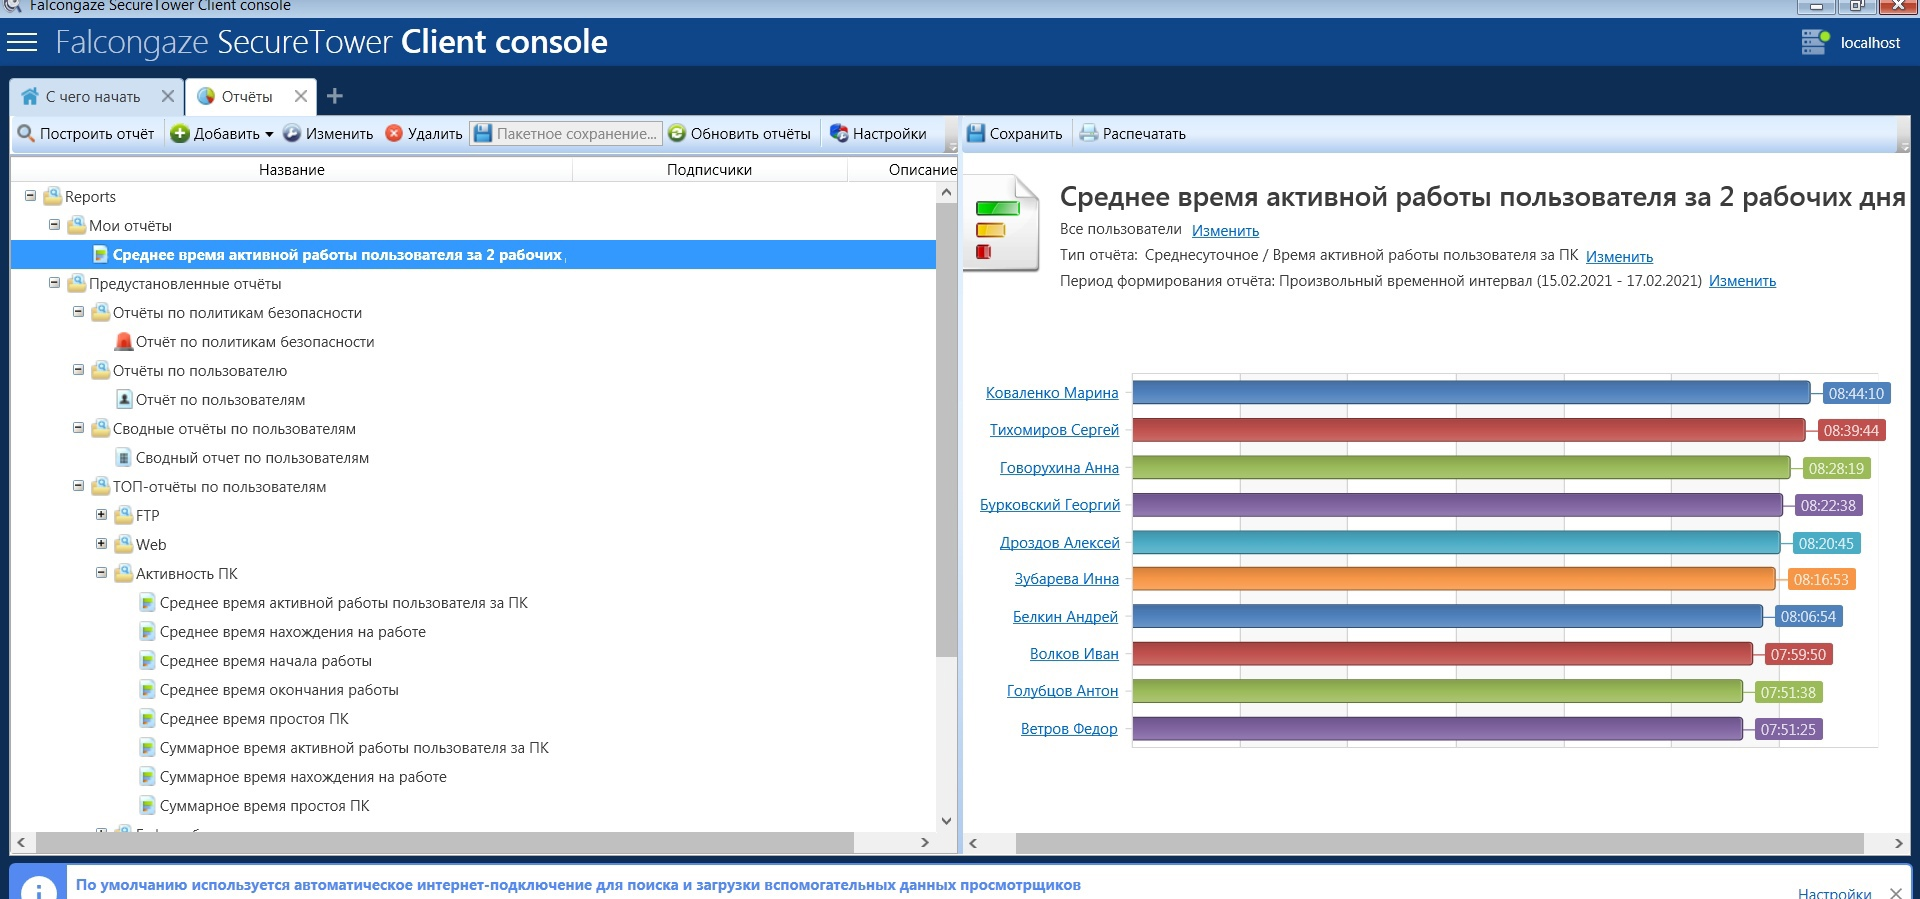
\includegraphics[scale=0.25]{pics/2.4.jpg}

        Дубликат "Среднее время активной работы пользователя за ПК"
    \end{center}

    \textbf{Пункт 2.8 - раздел отчета Активность пользователя за компьютером.} 
    \begin{center}
        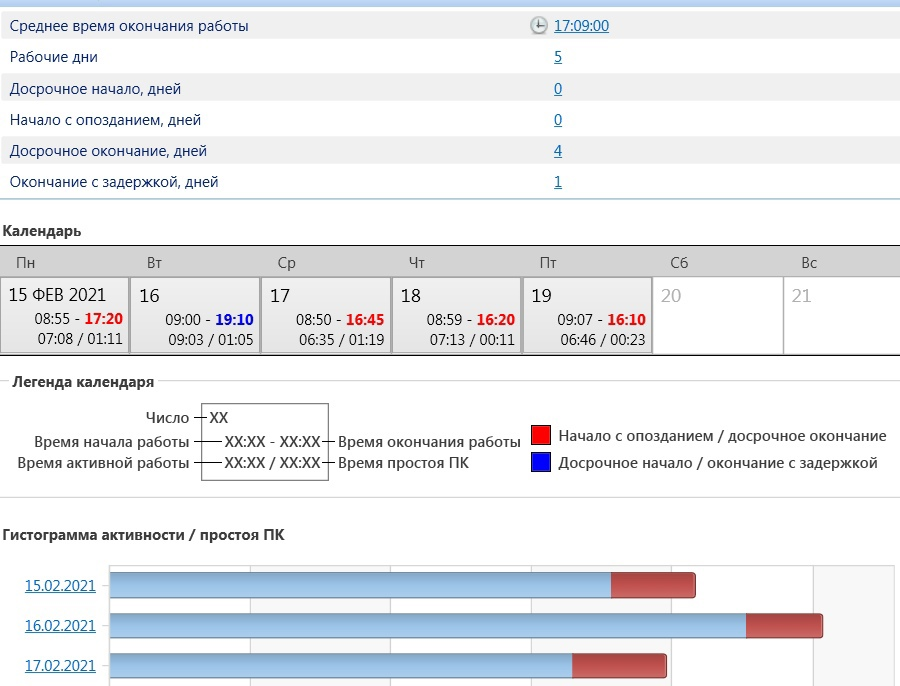
\includegraphics[scale=0.3]{pics/2.8.jpg}
        
        "Активность пользователя за компьютером."
    \end{center}

    \textbf{Пункт 2.9 - Сохранение отчета по пользователю Елана Кравцова.} 
    \begin{center}
        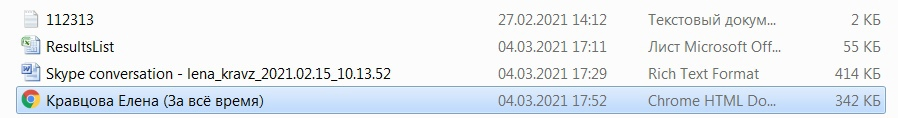
\includegraphics[scale=0.4]{pics/2.9.jpg}

        Отчет по пользователю сохранен
    \end{center}

    \vspace{-1.5em}
    \textbf{Пункт 3.2 - Поиск совпадений с файлами ранее созданного банка хэшей.} 
    \begin{center}
        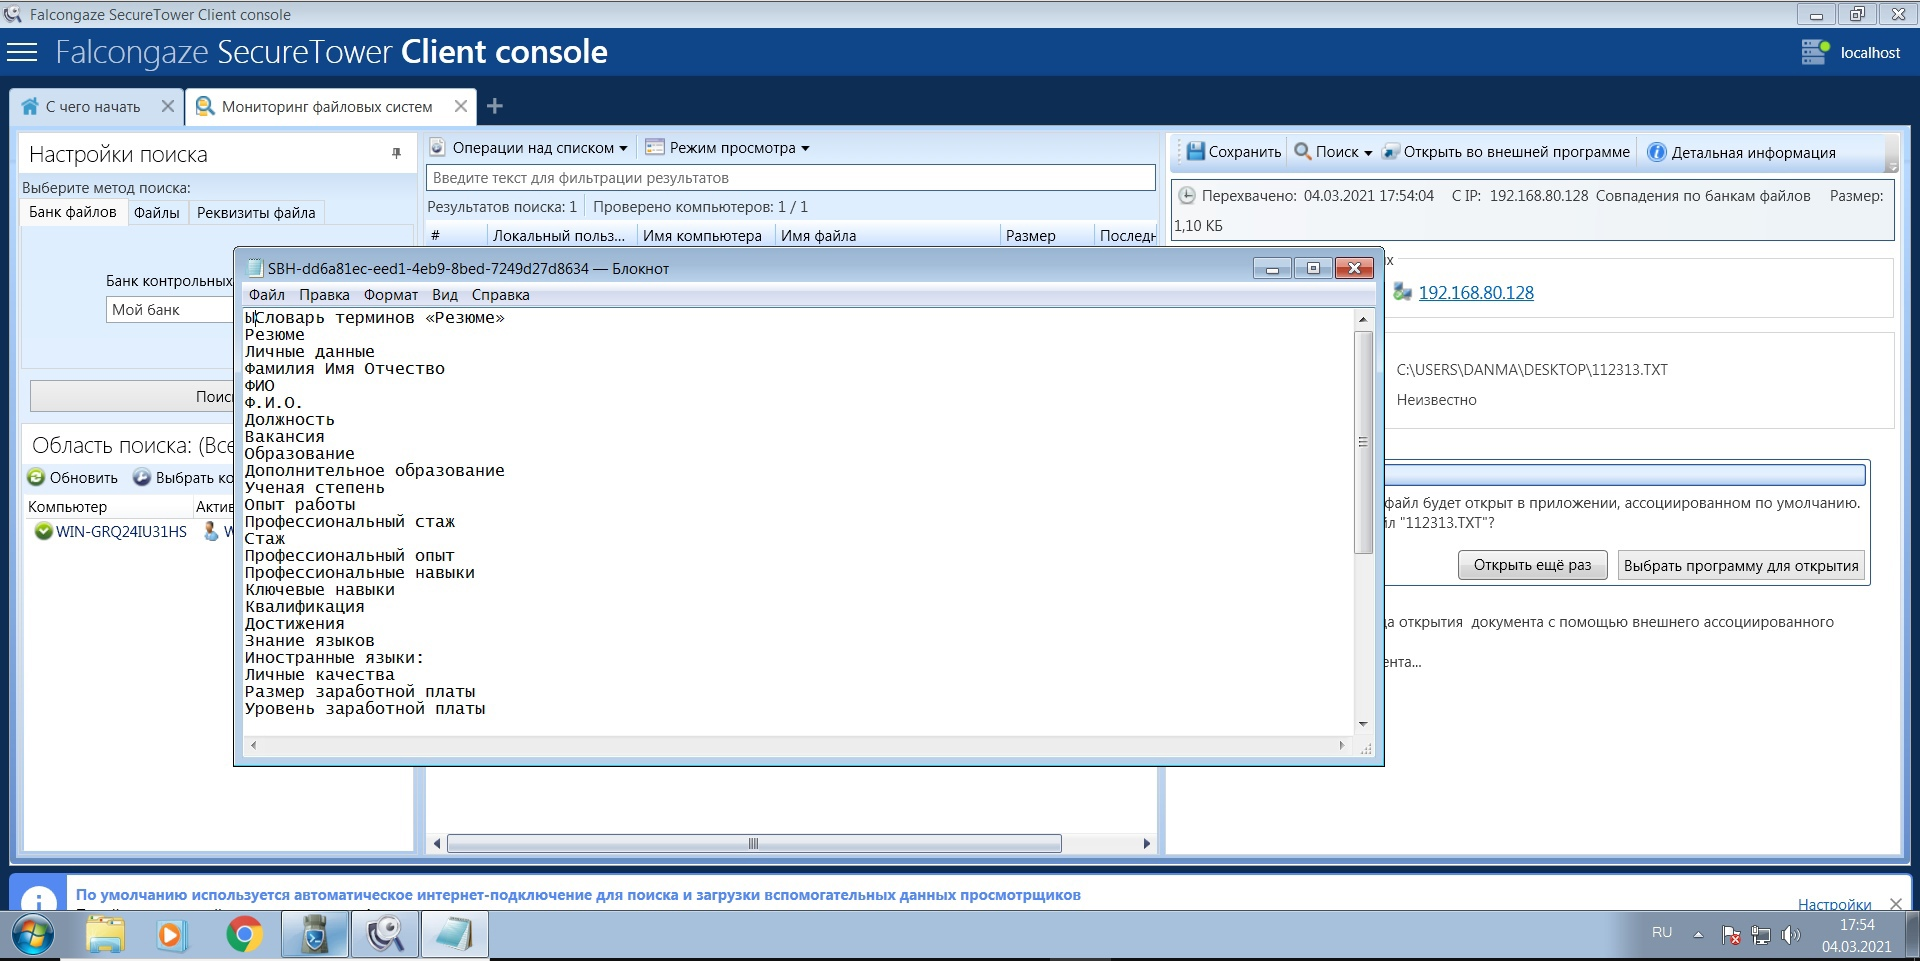
\includegraphics[scale=0.25]{pics/3.2.jpg}

        Найденный файл соответствует файлу-источнику, добавленному в банк
        хэшей при настройке индексирования ранее.
    \end{center}

    \vspace{-1.5em}
    \textbf{Пункт 3.4 - Поиск файла в файловой системе ПК.} 
    \begin{center}
        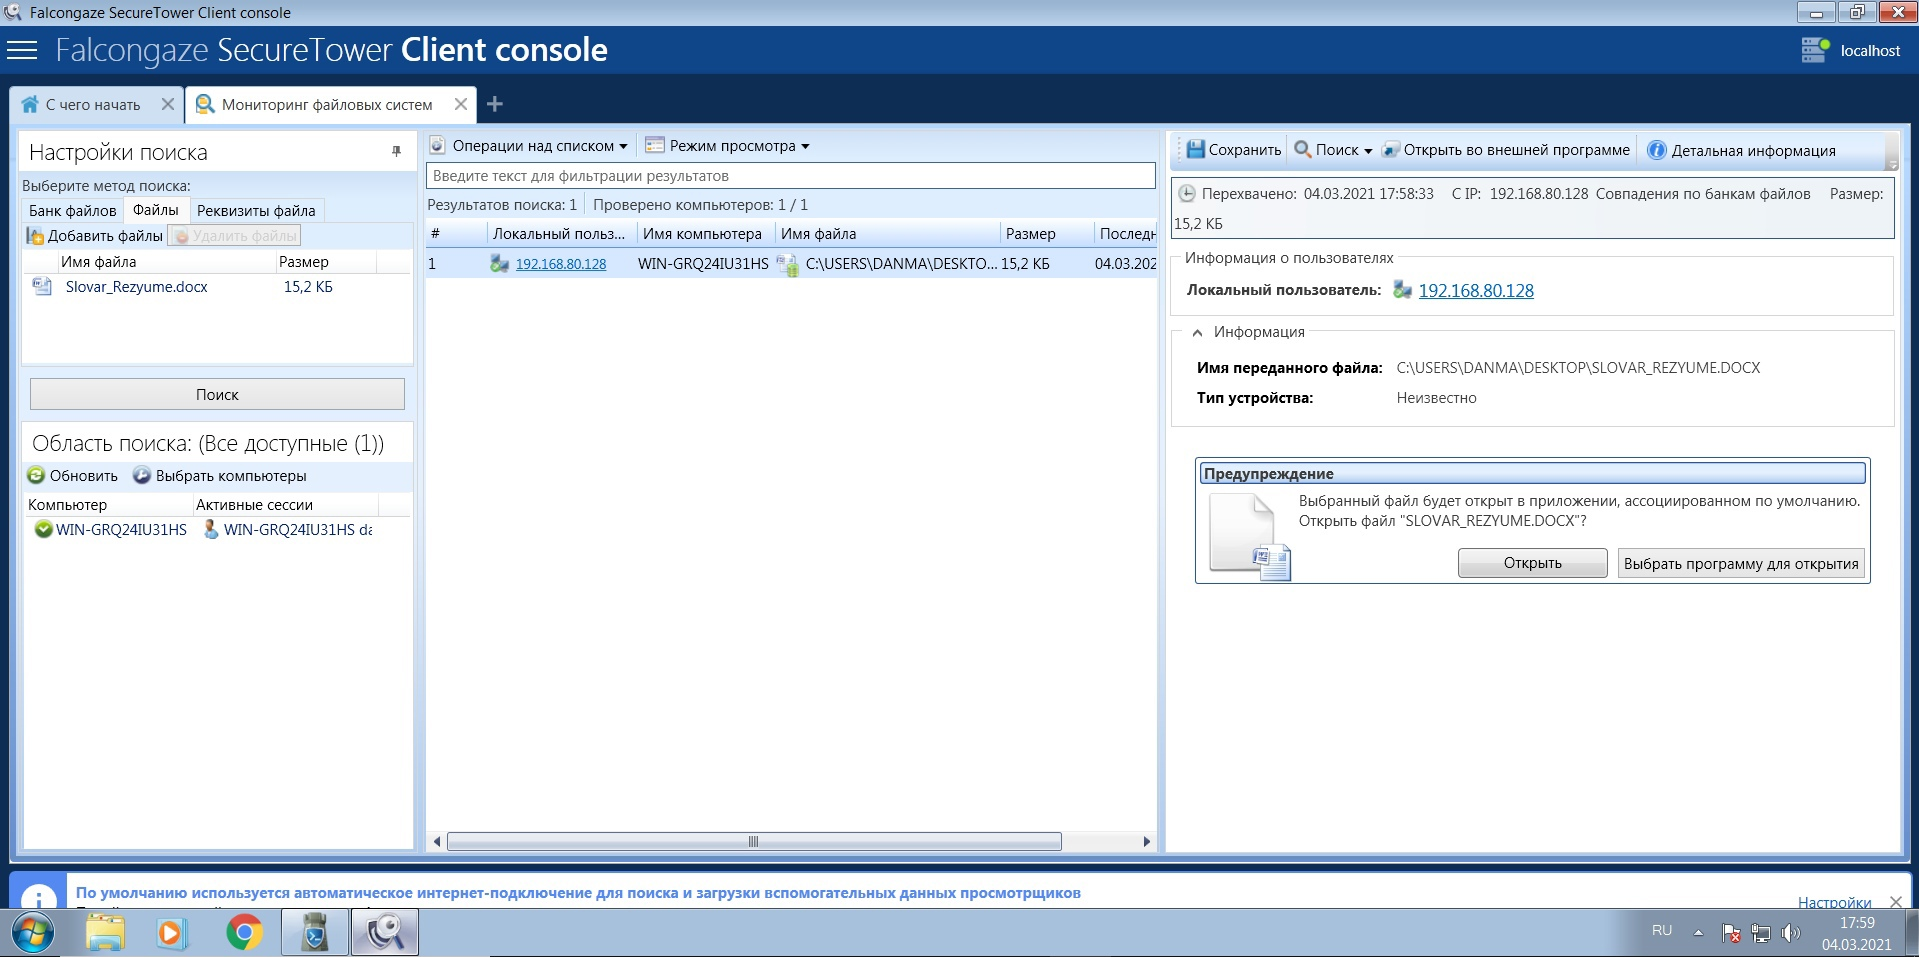
\includegraphics[scale=0.25]{pics/3.4.jpg}

        В ходе мониторинга найден файл Словарь резюме.docx, расположенный
        на рабочем столе в папке Student.
    \end{center}

    \newpage
    \textbf{Пункт 4.1 -  Активация видео-аудио мониторинга.} 
    \begin{center}
        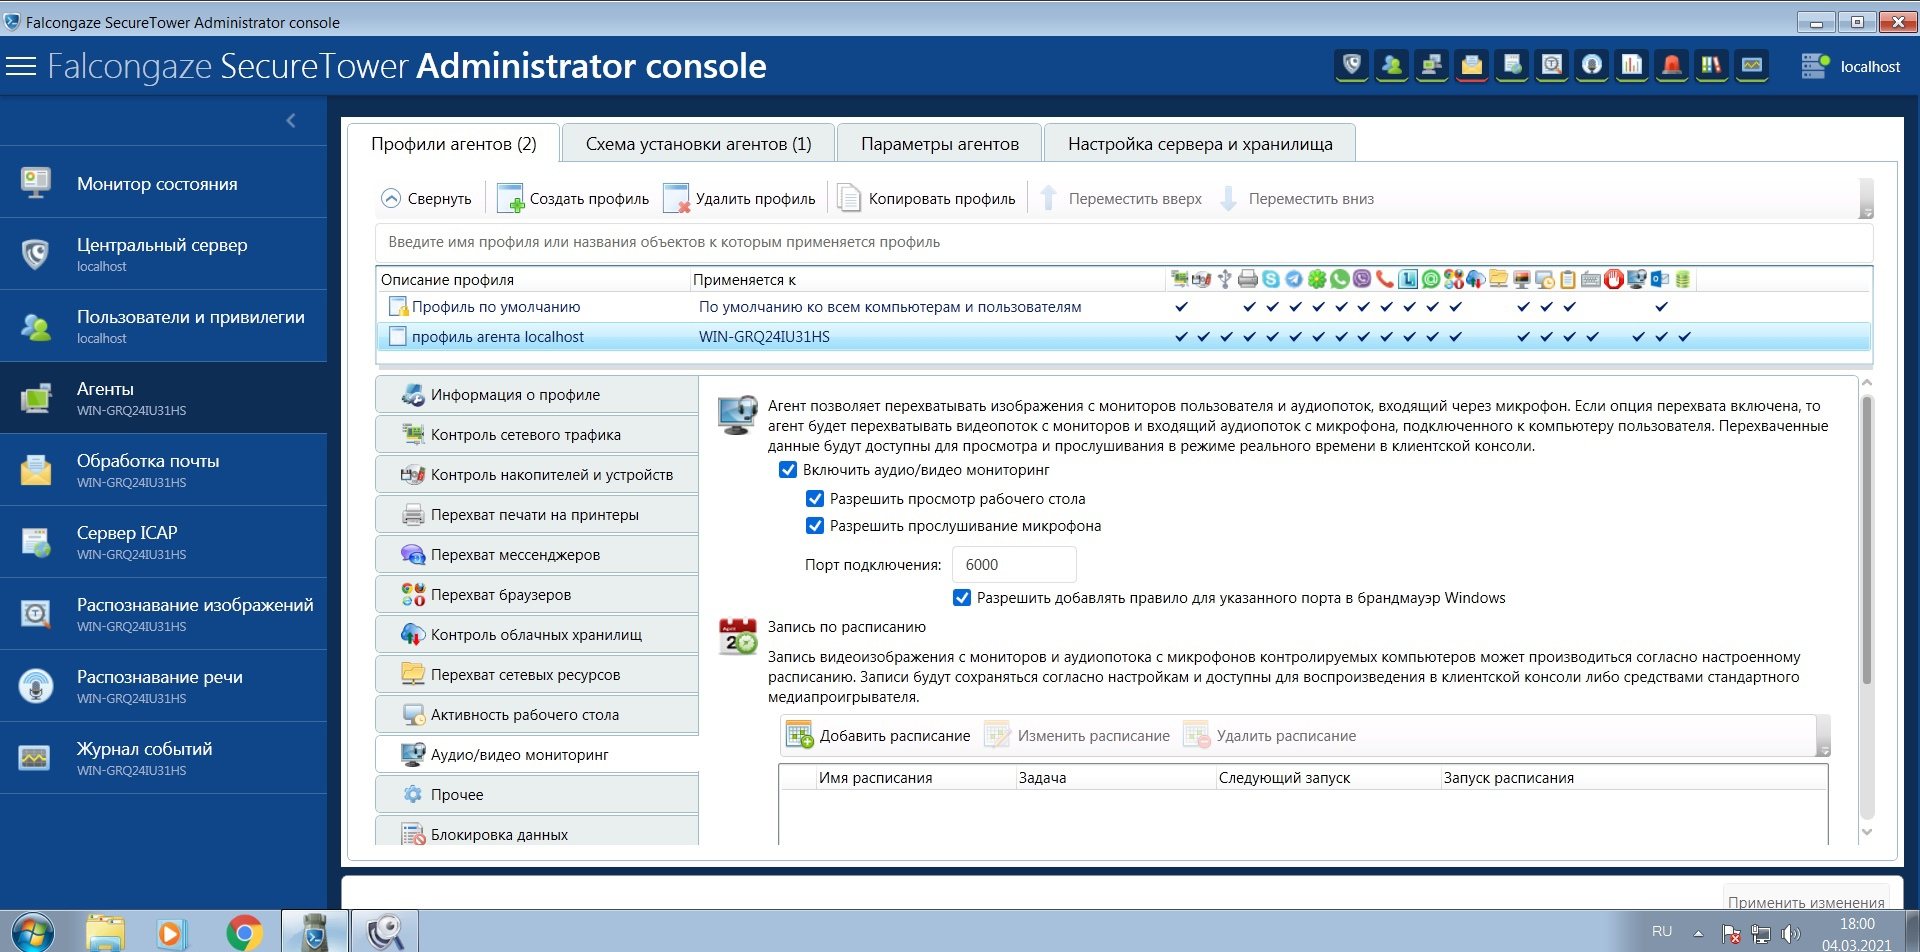
\includegraphics[scale=0.25]{pics/4.1.jpg}

        Мониторинг активирован.
    \end{center}

    \textbf{Пункт 4.8 - Изучение возможностей встроенного проигрывателя.}
    \begin{center}
        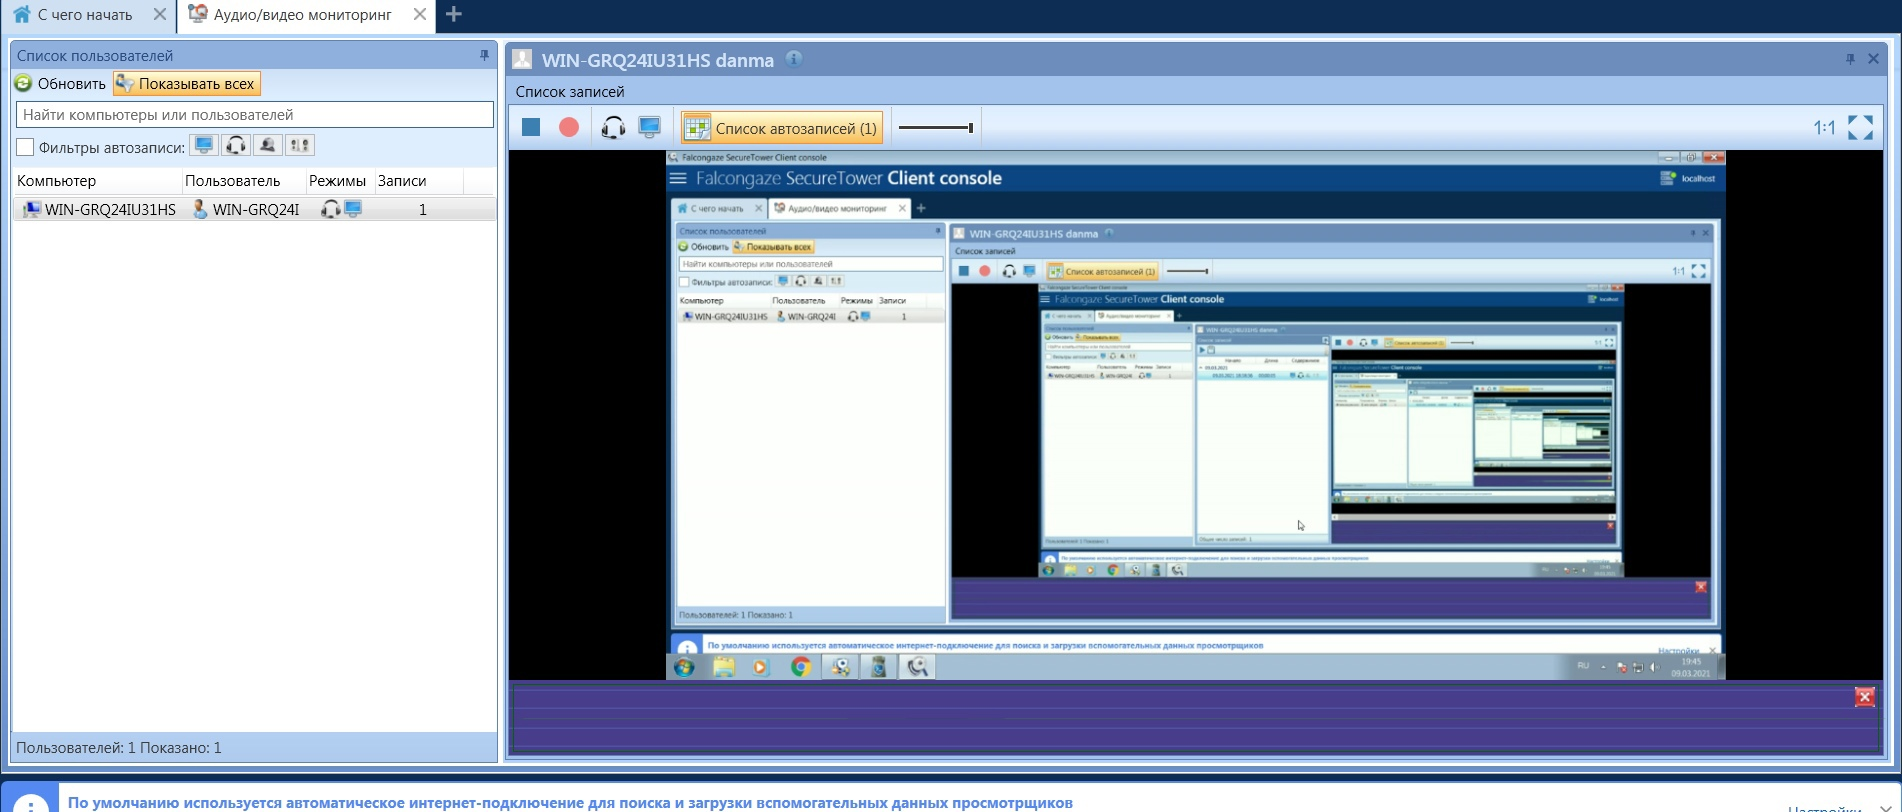
\includegraphics[scale=0.25]{pics/4.8.jpg}

        Воспроизводимое видео соответствуют действиям пользователя на
локальном компьютере.
    \end{center}

    \textbf{Пункт 4.9 - Отключение видео-аудио мониторинга, а также индексации.} 
    \begin{center}
        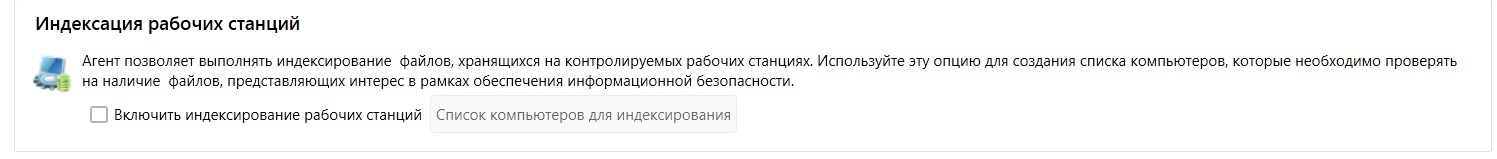
\includegraphics[scale=0.3]{pics/4.9.jpg}

         Индексация отключена 
    \end{center}

    \newpage
    \textbf{Выводы:}

    
    \textbf{Ответы на контрольные вопросы.}
    \begin{enumerate}
        \item \textbf{ Какой инструмент Консоли пользователя позволяет провести комплексный
    (и качественный и количественный) анализ статистики по выбранному направлению
    активности пользователя в сети? }

    \qquad Инструмент "Отчёты".
        \item \textbf{ Перечислите виды активности, по которым доступно построение
    статистических отчетов для отдельного пользователя сети организации. }

    \qquad Статистика перехвата данных, активность пользователя за компьютером, активность приложений,
    браузер-активность, статистика политик обеспечения безопасности.
        \item \textbf{ Как получить информацию о соблюдении режима рабочего дня
    пользователя? }

    \qquad "Отчёты" -> "Отчет по пользователю" -> "Активность пользователя за компьютером".
        \item \textbf{ Для чего выполняется индексирование файловых систем компьютеров? }

    \qquad Для возможности поиска по файлам.
        \item \textbf{ Возможно ли выполнить поиск произвольного файла в файловой системе
    контролируемого компьютера? Например, файла, выбранного пользователем, или с
    указанным именем или расширением. }

    \qquad Да, возможно.
        \item \textbf{ Возможно ли записать видео рабочего стола пользователя вручную? }

    \qquad Да, возможно.
        \item \textbf{ Позволяет ли система производить автоматическую запись результатов
    мониторинга компьютеров пользователей? }

    \qquad Да, позволяет.
    \end{enumerate}
    \end{document}